\section{Motivation} \label{Sec:Motivation}

This study was motivated by several scenarios which require syntax checking of RDF data as an input and ensuring of its quality. To mention one of such scenarios, let's discuss an example shown in {\it Figure \ref{Fig:Motivation}. The example describes a collaboration system for processing an input data, say for example to perform machine learning analysis. Of course,in a such case, a valid input data to the system is must. The input data is verified for further data processing. Most of the current existing systems  ensuring syntax-error-free RDF data, are stopped parsing at the first syntax error occurrence, as will be followed in Section \ref{Sec:Review}.
	\vspace{5mm} %5mm vertical space
\par
To stop parsing when the first syntax error is found will introduce much complications. Assuming, the input RDF data contains, for example, 10 syntax errors. Normally, what is happing when an error is found, the system will proceed with no further processing, instead it will report error's existence in the inserted data. The reported error then should be corrected by the user, then after correction data will be send back for re-checking of data's syntax. To make it more complex, imagine that the user will do such correction process for 10 times (remember that data includes 10 errors). Then, what if the data contains hundreds or thousands of errors. 
\vspace{5mm} %5mm vertical space
\begin{figure}[ht]
	\begin{center}
		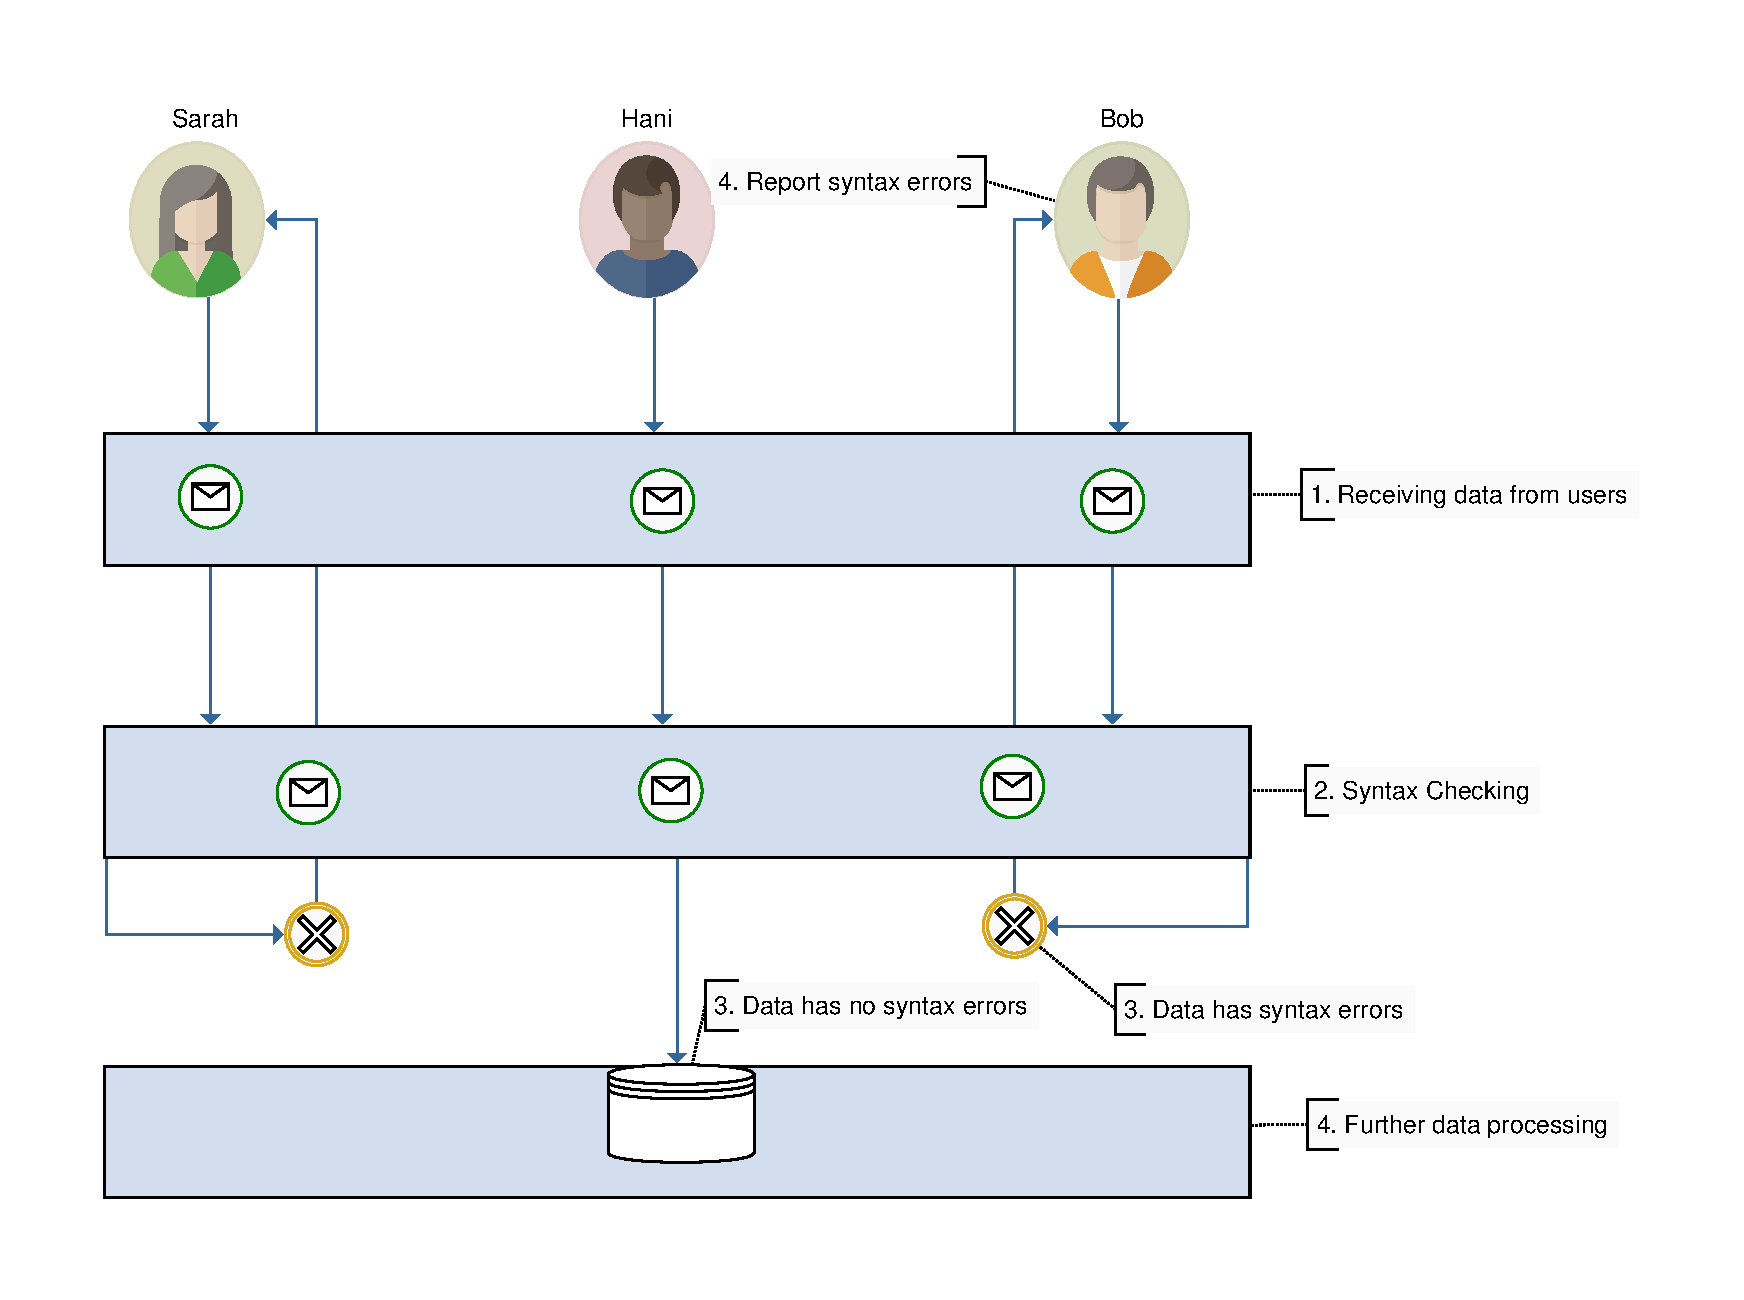
\includegraphics[scale=0.5,angle=0]{motivation}
		\caption{A motivation example of syntax checking of data before further processing}
		\label{Fig:Motivation}
	\end{center}
\end{figure}
let's dig deep to explain what is there in  {\it Figure \ref{Fig:Motivation}, It is showing a flow of data from clients or users seeking further data processing. 3 persons are shown in this Figure, their names are Bob, Hani, and Sarah. All of them start with the first phase by sending the data to be syntacticly checked. The parser starts checking if there syntax errors of the input data, then if such data passed with no syntax errors, it can be forwarded for further phases, i.e. for data processing, otherwise, the input data will send back to the user to correct the errors. {\it Figure \ref{Fig:Motivation} clearly shows that Sarah and Bob have syntax errors in their input data,then they got an error report, including found errors. In the meanwhile, Hani has received his data processed without getting such an error report, since his input data has no syntax errors. 
\vspace{5mm} %5mm vertical space
\par
This study has been encouraged by the illustrated example to find a suitable solution for such cases. The proposed solution will focus on producing a software program that can detect all or almost syntax errors that can be detected in the input data. 

